\documentclass[10pt, aspectratio=169]{beamer}

% ═══════════════════════════════════════════════════════════════════════════
%  Professional Academic Theme - IIT Delhi branding
% ═══════════════════════════════════════════════════════════════════════════

% ── Theme ───────────────────────────────────────────────────────────────────
\usetheme{Madrid}
\useinnertheme{rectangles}
\beamertemplatenavigationsymbolsempty

% ── Colour Palette ─────────────────────────────────────────────────────────
\definecolor{iitdNavy}{HTML}{003B5C}
\definecolor{iitdDark}{HTML}{002642}
\definecolor{iitdAccent}{HTML}{0077B6}
\definecolor{iitdGray}{HTML}{4A5568}
\definecolor{iitdLightGray}{HTML}{E2E8F0}
\definecolor{alertRed}{HTML}{B91C1C}
\definecolor{successGreen}{HTML}{047857}

% ── Apply colours ──────────────────────────────────────────────────────────
\setbeamercolor{palette primary}{bg=iitdNavy, fg=white}
\setbeamercolor{palette secondary}{bg=iitdDark, fg=white}
\setbeamercolor{palette tertiary}{bg=iitdDark, fg=white}
\setbeamercolor{palette quaternary}{bg=iitdNavy, fg=white}
\setbeamercolor{structure}{fg=iitdNavy}
\setbeamercolor{frametitle}{bg=iitdNavy, fg=white}
\setbeamercolor{title}{fg=white, bg=iitdNavy}
\setbeamercolor{subtitle}{fg=iitdLightGray}
\setbeamercolor{author}{fg=white}
\setbeamercolor{institute}{fg=iitdLightGray}
\setbeamercolor{date}{fg=iitdLightGray}
\setbeamercolor{normal text}{fg=iitdGray}
\setbeamercolor{alerted text}{fg=alertRed}
\setbeamercolor{example text}{fg=successGreen}
\setbeamercolor{block title}{bg=iitdNavy, fg=white}
\setbeamercolor{block body}{bg=iitdLightGray!40, fg=iitdGray}
\setbeamercolor{block title alerted}{bg=alertRed!85!black, fg=white}
\setbeamercolor{block body alerted}{bg=alertRed!8, fg=iitdGray}
\setbeamercolor{block title example}{bg=successGreen!85!black, fg=white}
\setbeamercolor{block body example}{bg=successGreen!8, fg=iitdGray}
\setbeamercolor{itemize item}{fg=iitdNavy}
\setbeamercolor{itemize subitem}{fg=iitdAccent}
\setbeamercolor{enumerate item}{fg=iitdNavy}

% ── Fonts ──────────────────────────────────────────────────────────────────
\setbeamerfont{title}{size=\Large, series=\bfseries}
\setbeamerfont{frametitle}{size=\large, series=\bfseries}
\setbeamerfont{block title}{size=\normalsize, series=\bfseries}

% ── Bullets ────────────────────────────────────────────────────────────────
\setbeamertemplate{itemize item}{\small$\bullet$}
\setbeamertemplate{itemize subitem}{\scriptsize$\circ$}

% ── Footer ─────────────────────────────────────────────────────────────────
\setbeamertemplate{footline}{%
  \hfill%
  \usebeamercolor[fg]{normal text}%
  \usebeamerfont{footline}%
  \footnotesize\insertframenumber\,/\,\inserttotalframenumber%
  \hspace{8pt}\vspace{4pt}%
}

% ── Packages ───────────────────────────────────────────────────────────────
\usepackage{graphicx}
\usepackage{booktabs}
\usepackage[table]{xcolor}
\usepackage{amsmath,amssymb}
\usepackage{tikz}
\usetikzlibrary{positioning}
\usepackage{hyperref}
\usepackage{multicol}
\usepackage{caption}
\captionsetup{font=small, labelformat=empty}

\newcommand{\rupee}{\textrm{Rs.}\,}

% ── Key Insight box ────────────────────────────────────────────────────────
\newcommand{\keyinsight}[1]{%
  \begin{beamercolorbox}[wd=\textwidth, sep=6pt, rounded=true]{block body}
    \textcolor{iitdNavy}{\textbf{\small$\star$\;Key Insight:}}\;
    {\small #1}
  \end{beamercolorbox}%
}

% ═══════════════════════════════════════════════════════════════════════════
\begin{document}

% ─── SLIDE 1: TITLE ──────────────────────────────────────────────────────────
\begin{frame}[plain]
    \begin{tikzpicture}[remember picture, overlay]
        \shade[left color=iitdDark, right color=iitdAccent!80!iitdNavy,
               shading angle=15]
            (current page.south west) rectangle (current page.north east);
        \fill[white, opacity=0.06]
            ([xshift=-2cm, yshift=-2.5cm]current page.north east) circle (6cm);
        \fill[white, opacity=0.04]
            ([xshift=2.5cm, yshift=2cm]current page.south west) circle (4.5cm);
        \draw[iitdAccent!60!white, line width=0.8pt]
            ([xshift=2cm, yshift=-0.5cm]current page.west)
            -- ([xshift=-2cm, yshift=-0.5cm]current page.east);

        \node[anchor=south, text width=0.85\paperwidth, align=center]
            at ([yshift=1.0cm]current page.center) {
                {\LARGE\bfseries\color{white}%
                 Ecological Evaluation of Sunder Nursery}\\[10pt]
                {\large\color{iitdLightGray}Using the Contingent Valuation Method}\\[14pt]
                {\large\color{iitdAccent!80!white}\textbf{RDL725 - Field Assignment}}
            };

        \node[anchor=north, text width=0.75\paperwidth, align=center]
            at ([yshift=-1.2cm]current page.center) {
                {\normalsize\color{white}%
                 \textbf{Prem Bhugra}\;\;|\;\;%
                 \textbf{Sakhare Yash Balram}\;\;|\;\;%
                 \textbf{Ninad Narsing Gawade}\;\;|\;\;%
                 \textbf{Nitin Verma}}\\[10pt]
                {\normalsize\color{iitdLightGray}%
                 Course Coordinator: \textbf{Prof.\ Vivek Kumar}}\\[4pt]
                {\small\color{iitdLightGray}%
                 TAs: Nandita Pawar, Rahul Dwivedi}\\[6pt]
                {\small\color{iitdLightGray}%
                 Department of Chemical Engineering\\
                 Indian Institute of Technology Delhi}
            };
    \end{tikzpicture}
\end{frame}

% ─── SLIDE 2: OUTLINE ─────────────────────────────────────────────────────────
\begin{frame}{Outline}
    \begin{columns}[T]
        \begin{column}{0.48\textwidth}
            \begin{enumerate}
                \item Introduction \& Motivation
                \item About Sunder Nursery
                \item Theoretical Framework
                \item Survey Methodology
                \item Demographic Profile
            \end{enumerate}
        \end{column}
        \begin{column}{0.48\textwidth}
            \begin{enumerate}
                \setcounter{enumi}{5}
                \item CVM Results: Willingness to Pay
                \item Non-Use Value Analysis
                \item TCM Results: Consumer Surplus
                \item Total Economic Value
                \item Discussion \& Conclusion
            \end{enumerate}
        \end{column}
    \end{columns}
\end{frame}

% ═══════════════════════════════════════════════════════════════════════════
\section{Introduction}
% ═══════════════════════════════════════════════════════════════════════════

% ─── SLIDE 3: INTRODUCTION ─────────────────────────────────────────────────
\begin{frame}{Introduction: Why Value the Environment?}
    \begin{columns}[T]
        \begin{column}{0.55\textwidth}
            \textbf{The Problem:}
            \begin{itemize}
                \item Urban parks and heritage sites provide enormous benefits: recreation, ecological balance, cultural preservation, aesthetic pleasure
                \item These benefits have \textbf{no market price}
                \item Policy-makers tend to undervalue what they cannot price
            \end{itemize}

            \vspace{0.6em}
            \textbf{Our Objective:}
            \begin{itemize}
                \item Estimate the \textbf{Total Economic Value (TEV)} of Sunder Nursery using CVM and TCM
                \item Capture both \textbf{use values} (recreation) and \textbf{non-use values} (bequest, existence)
            \end{itemize}
        \end{column}
        \begin{column}{0.42\textwidth}
            \begin{block}{Field Visit Details}
                \small
                \begin{itemize}
                    \item \textbf{Site:} Sunder Nursery, New Delhi
                    \item \textbf{Date:} Friday, 10 April 2026
                    \item \textbf{Time:} 4:00 PM - 7:30 PM
                    \item \textbf{Sample:} 45 visitors surveyed
                    \item \textbf{Method:} Bilingual Google Forms (English-Hindi)
                \end{itemize}
            \end{block}
        \end{column}
    \end{columns}
\end{frame}

% ═══════════════════════════════════════════════════════════════════════════
\section{Site Description}
% ═══════════════════════════════════════════════════════════════════════════

% ─── SLIDE 4: SUNDER NURSERY ─────────────────────────────────────────────
\begin{frame}{About Sunder Nursery}
    \begin{columns}[T]
        \begin{column}{0.50\textwidth}
            \textbf{History \& Restoration:}
            \begin{itemize}
                \small
                \item 90-acre heritage park in Nizamuddin, adjacent to Humayun's Tomb (UNESCO)
                \item Origins in the 16th century as a Mughal-era nursery
                \item Restored by \textbf{Aga Khan Trust for Culture} (2007-2018)
                \item Reopened in \textbf{February 2018}
            \end{itemize}

            \vspace{0.4em}
            \textbf{Ecological Features:}
            \begin{itemize}
                \small
                \item 300+ tree species, 80+ flowering varieties
                \item 80+ bird species recorded
                \item 6 restored Mughal-era monuments
                \item Restored water channels \& wetlands
            \end{itemize}
        \end{column}
        \begin{column}{0.47\textwidth}
            \begin{figure}
                \centering
                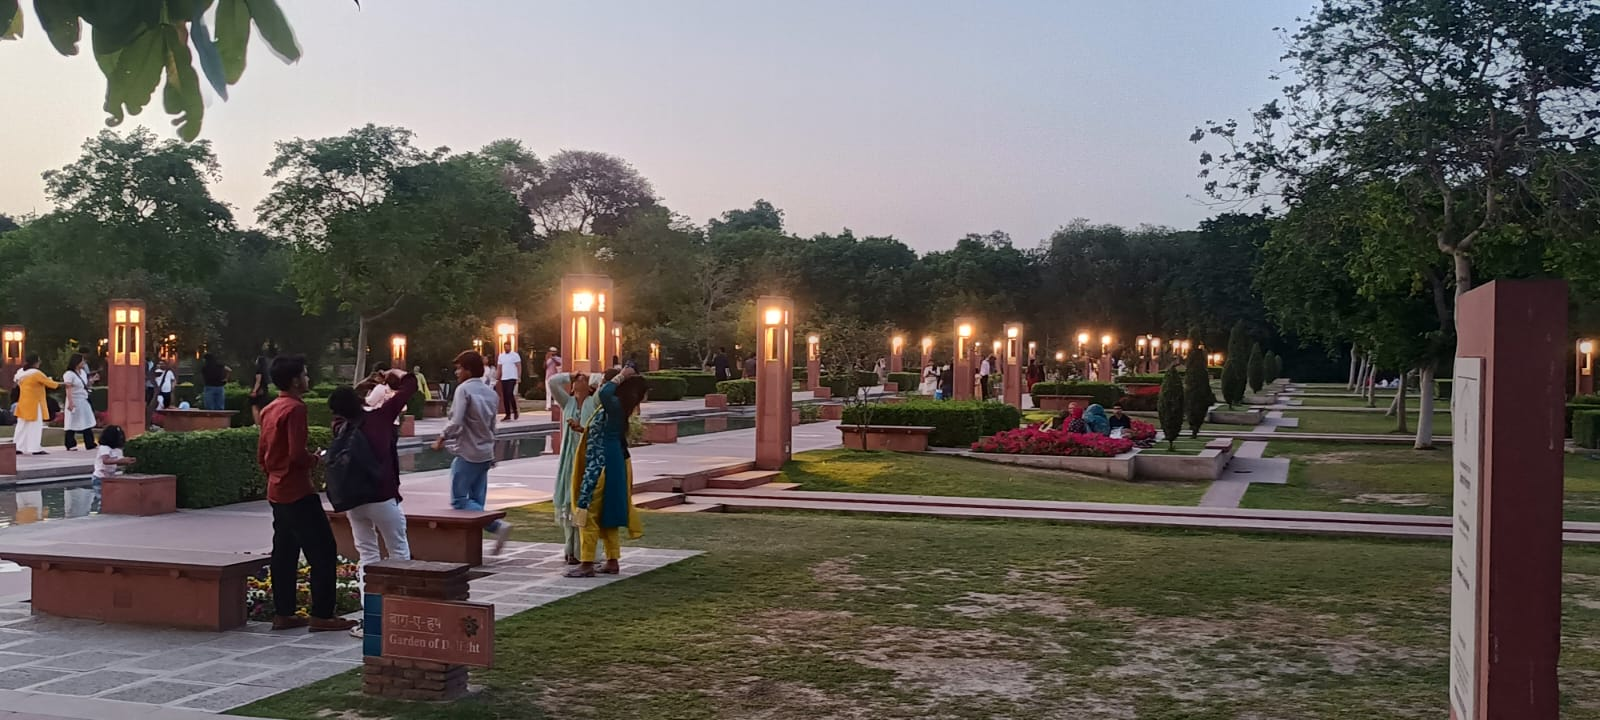
\includegraphics[width=0.95\linewidth, height=3.2cm, keepaspectratio=false]{../Images/1.jpeg}
                \caption{Garden of Delight at dusk}
            \end{figure}
            \vspace{-0.5em}
            \begin{figure}
                \centering
                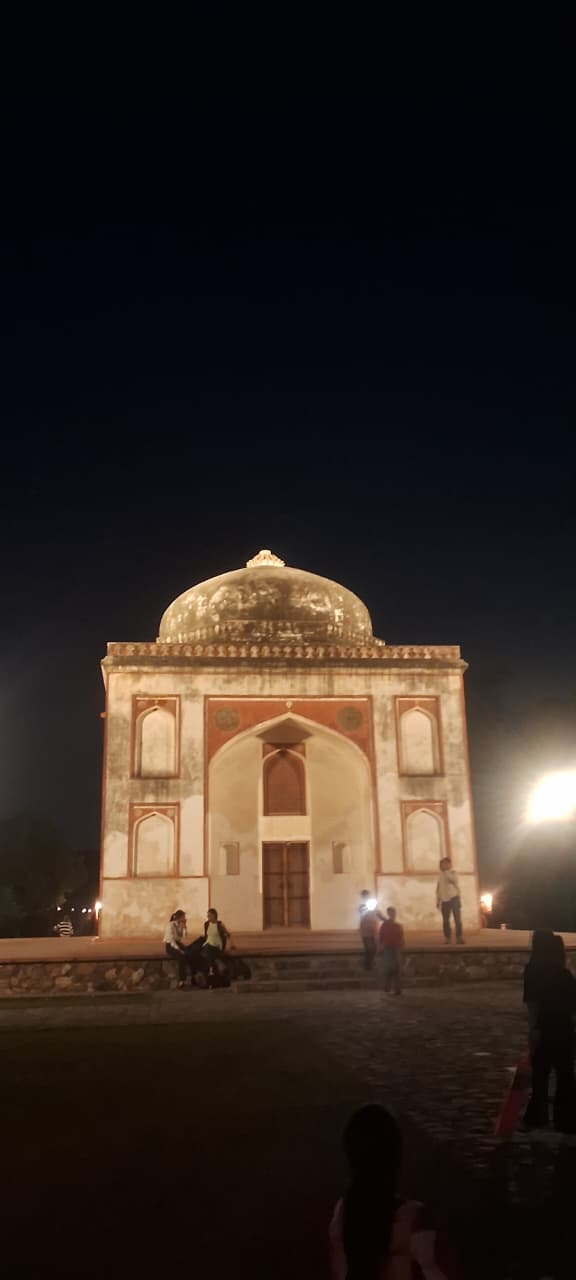
\includegraphics[width=0.95\linewidth, height=3.2cm, keepaspectratio=false]{../Images/4.jpeg}
                \caption{Sundarwala Burj at night}
            \end{figure}
        \end{column}
    \end{columns}
\end{frame}

% ═══════════════════════════════════════════════════════════════════════════
\section{Theoretical Framework}
% ═══════════════════════════════════════════════════════════════════════════

% ─── SLIDE 5: THEORETICAL FRAMEWORK ───────────────────────────────────────
\begin{frame}{Theoretical Framework}
    \begin{columns}[T]
        \begin{column}{0.50\textwidth}
            \textbf{Total Economic Value (TEV):}
            \[
                \text{TEV} = \underbrace{\text{Use Value}}_{\text{direct benefit}} + \underbrace{\text{Non-Use Value}}_{\text{option + bequest + existence}}
            \]

            \vspace{0.3em}
            \begin{itemize}
                \small
                \item \textbf{Use Value:} Walking, picnicking, birdwatching
                \item \textbf{Option Value:} Keeping the option to visit in the future
                \item \textbf{Bequest Value:} Preserving for future generations
                \item \textbf{Existence Value:} Knowing the park exists and is protected
            \end{itemize}
        \end{column}
        \begin{column}{0.47\textwidth}
            \begin{block}{Contingent Valuation Method (CVM)}
                \small
                \textbf{Stated-preference technique:}\\
                Creates a hypothetical market via survey; asks WTP for conservation\\[4pt]
                Payment vehicle: \textit{Increased entry fee}
            \end{block}

            \vspace{0.4em}
            \begin{block}{Travel Cost Method (TCM)}
                \small
                \textbf{Revealed-preference technique:}\\
                Infers value from actual travel expenditure\\[4pt]
                Consumer surplus = benefit above actual spend
            \end{block}
        \end{column}
    \end{columns}
\end{frame}

% ═══════════════════════════════════════════════════════════════════════════
\section{Methodology}
% ═══════════════════════════════════════════════════════════════════════════

% ─── SLIDE 6: SURVEY DESIGN ──────────────────────────────────────────────
\begin{frame}{Survey Design \& Data Collection}
    \begin{columns}[T]
        \begin{column}{0.50\textwidth}
            \textbf{Questionnaire Structure (16 questions):}
            \begin{enumerate}
                \small
                \item \textbf{CVM Core:} Aspects valued + WTP (Yes/No)
                \item \textbf{Contribution:} Max extra amount (Rs.\ 10/20/50/100)
                \item \textbf{Protest Feedback:} Why not willing
                \item \textbf{Non-Use Values:} Bequest importance + existence value + ecological rating
                \item \textbf{TCM Core:} Transport mode, travel cost, travel time, sole destination
                \item \textbf{Demographics:} Frequency, age, income
            \end{enumerate}

            \vspace{0.3em}
            \keyinsight{Skip logic directed WTP=Yes to amount page, WTP=No to protest page.}
        \end{column}
        \begin{column}{0.47\textwidth}
            \begin{figure}
                \centering
                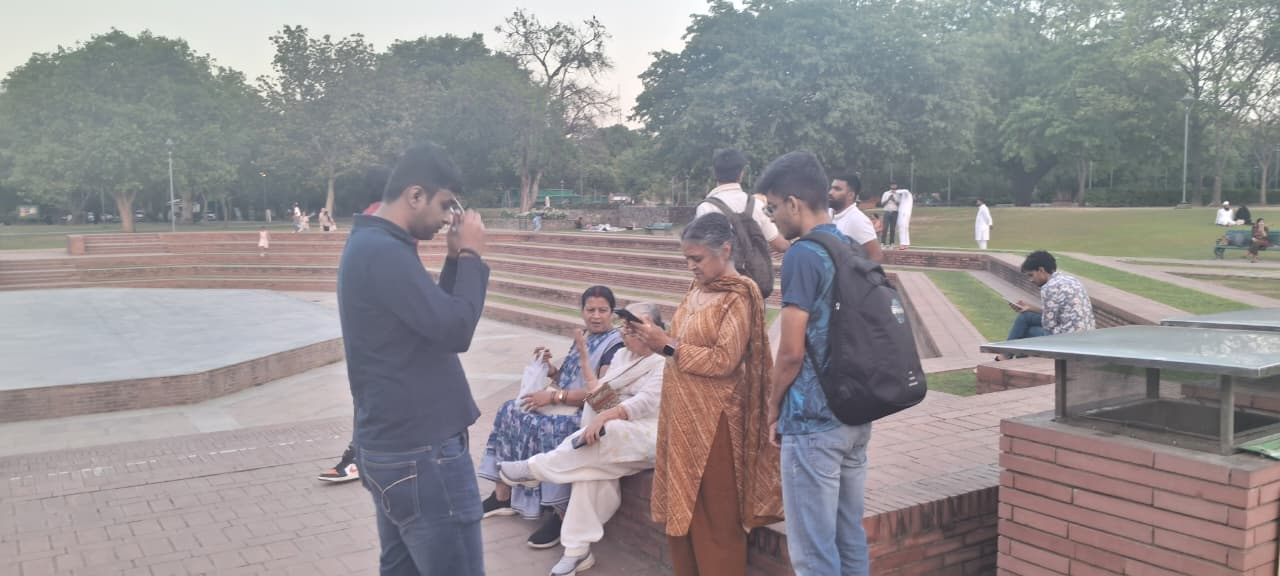
\includegraphics[width=0.95\linewidth]{../Images/Review 6.jpeg}
                \caption{Conducting the survey on-site}
            \end{figure}
            \vspace{-0.5em}
            \begin{figure}
                \centering
                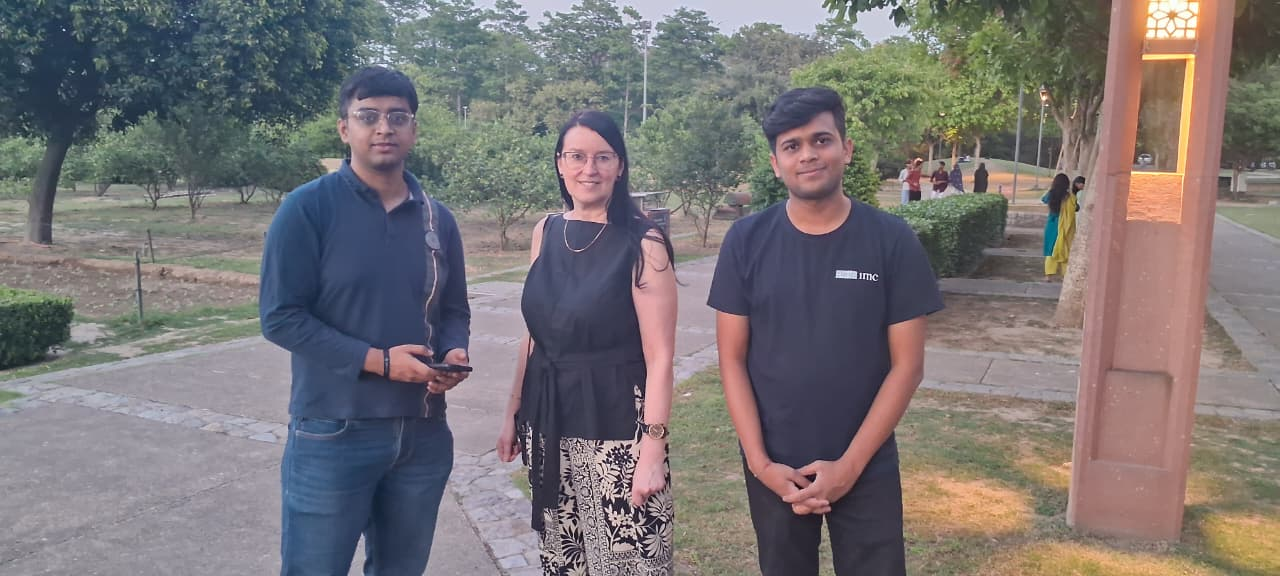
\includegraphics[width=0.95\linewidth]{../Images/Review 7.jpeg}
                \caption{Surveying a visitor near the garden}
            \end{figure}
        \end{column}
    \end{columns}
\end{frame}

% ═══════════════════════════════════════════════════════════════════════════
\section{Results}
% ═══════════════════════════════════════════════════════════════════════════

% ─── SLIDE 7: DEMOGRAPHICS ───────────────────────────────────────────────
\begin{frame}{Respondent Demographics (n = 45)}
    \begin{columns}[T]
        \begin{column}{0.48\textwidth}
            \begin{figure}
                \centering
                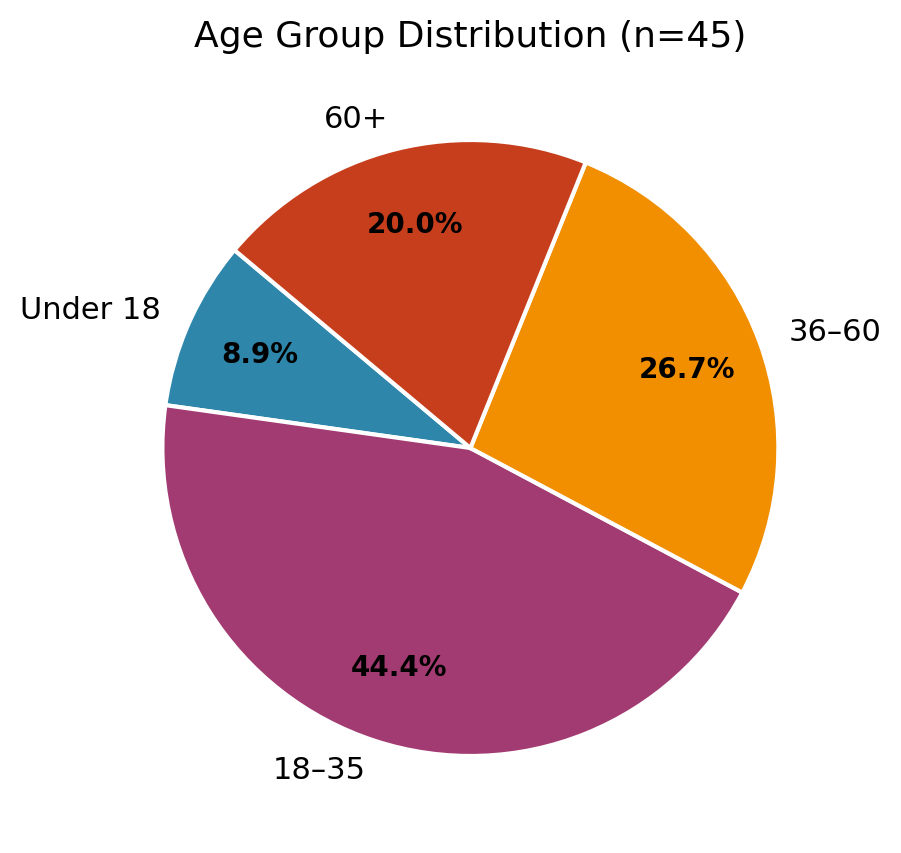
\includegraphics[width=\linewidth]{../report/figures/01_age_distribution.png}
                \caption{Age group distribution}
            \end{figure}
        \end{column}
        \begin{column}{0.48\textwidth}
            \begin{figure}
                \centering
                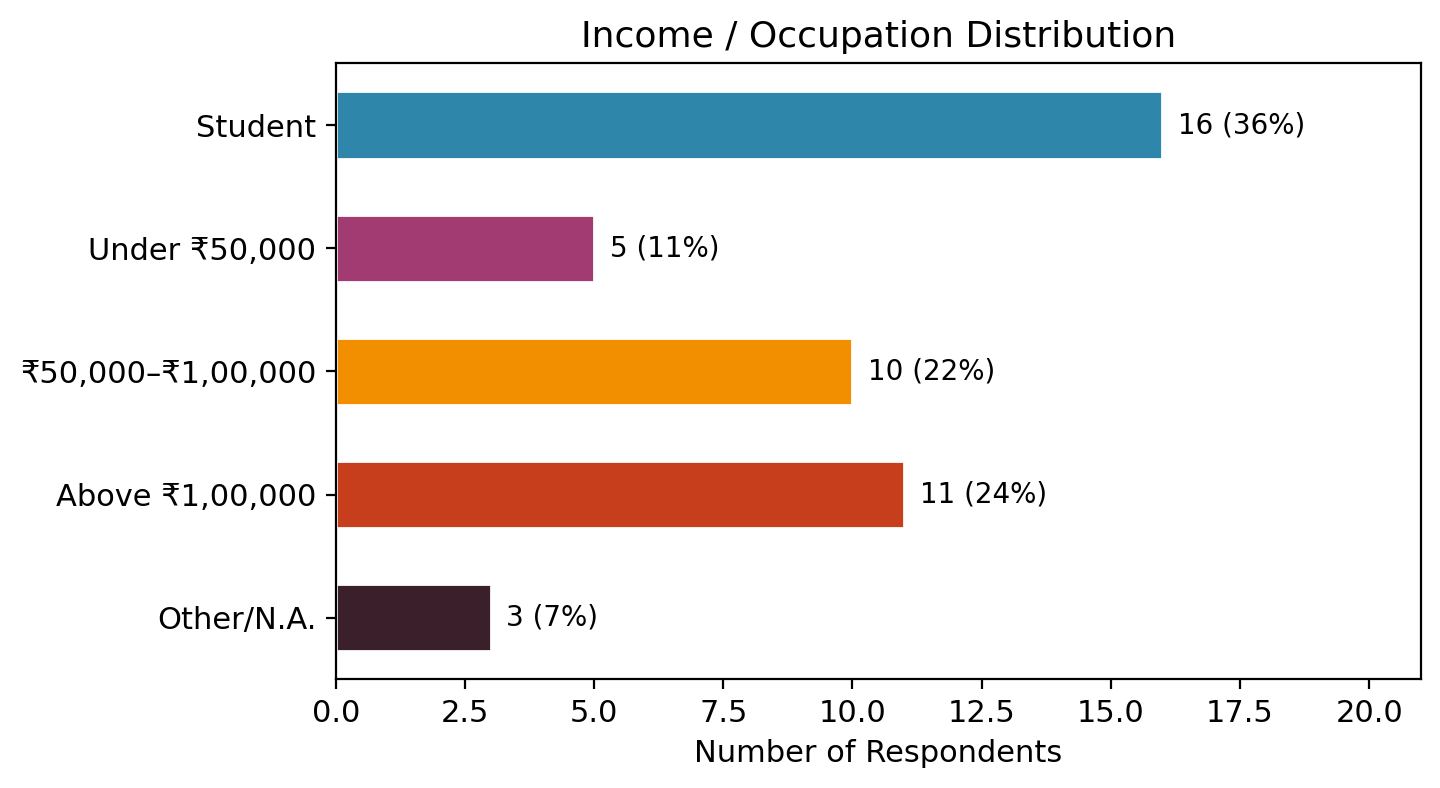
\includegraphics[width=\linewidth]{../report/figures/02_income_distribution.png}
                \caption{Income/occupation distribution}
            \end{figure}
        \end{column}
    \end{columns}

    \vspace{0.3em}
    \keyinsight{Largest groups: 18-35 age bracket (44.4\%) and students (35.6\%). 35.6\% were first-time visitors.}
\end{frame}

% ─── SLIDE 8: ASPECTS VALUED ─────────────────────────────────────────────
\begin{frame}{What Do Visitors Value Most?}
    \begin{columns}[T]
        \begin{column}{0.55\textwidth}
            \begin{figure}
                \centering
                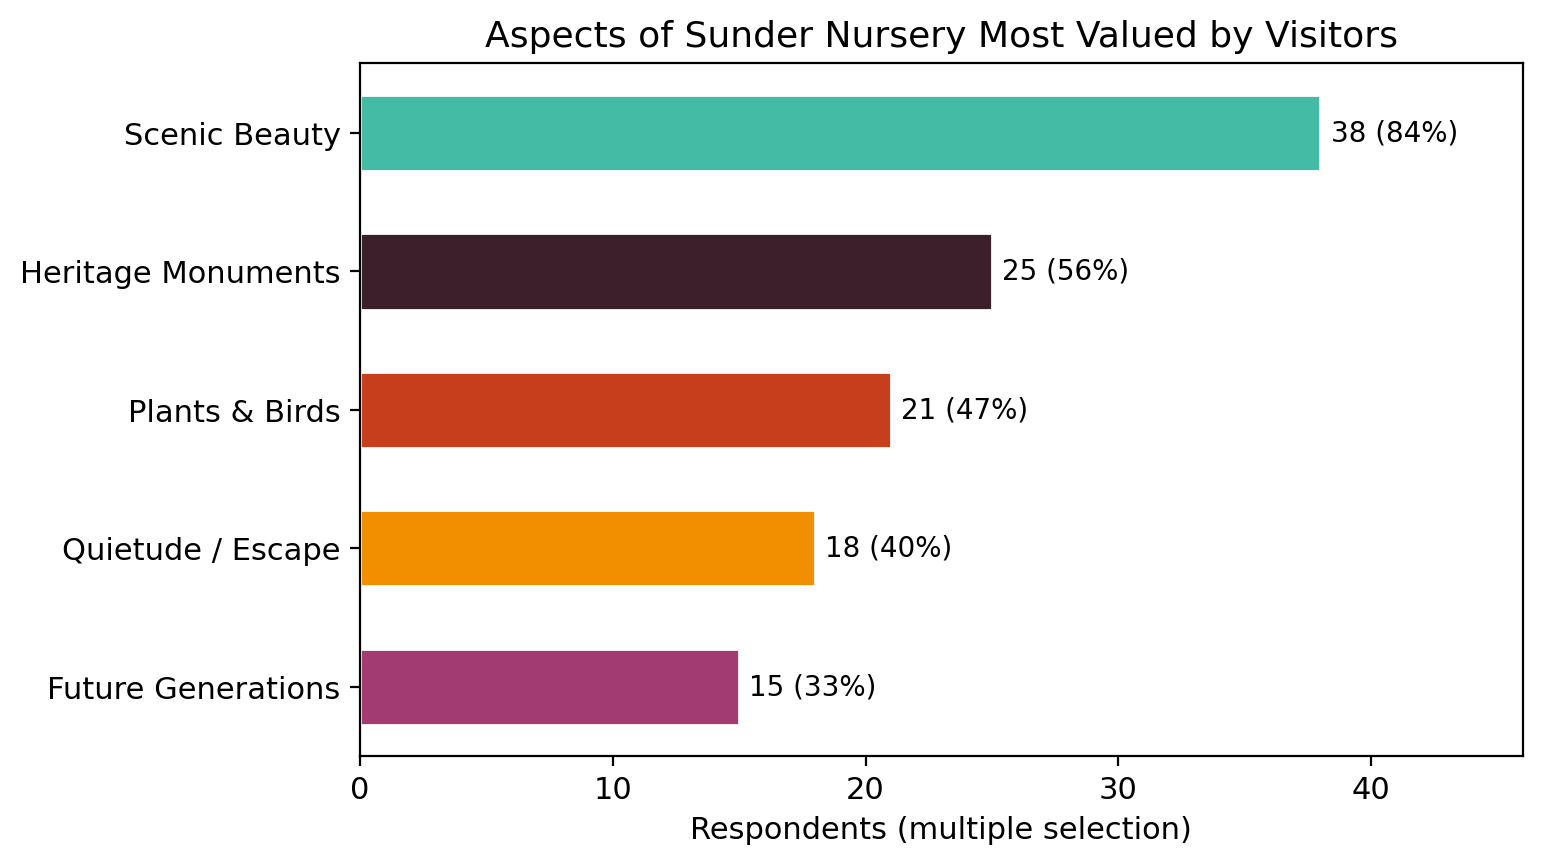
\includegraphics[width=\linewidth]{../report/figures/04_aspects_valued.png}
                \caption{Aspects of Sunder Nursery most valued}
            \end{figure}
        \end{column}
        \begin{column}{0.42\textwidth}
            \textbf{Top aspects (multiple selections):}
            \begin{enumerate}
                \small
                \item Scenic beauty: \textbf{84.4\%}
                \item Heritage monuments: \textbf{55.6\%}
                \item Plants \& birds: \textbf{46.7\%}
                \item Quietude/escape: \textbf{40.0\%}
                \item Future generations: \textbf{33.3\%}
            \end{enumerate}

            \vspace{0.5em}
            \keyinsight{A third of visitors explicitly valued ``availability for future generations'' - a strong signal of latent bequest value.}
        \end{column}
    \end{columns}
\end{frame}

% ─── SLIDE 9: WTP RESULTS ────────────────────────────────────────────────
\begin{frame}{CVM Results: Willingness to Pay}
    \begin{columns}[T]
        \begin{column}{0.45\textwidth}
            \begin{figure}
                \centering
                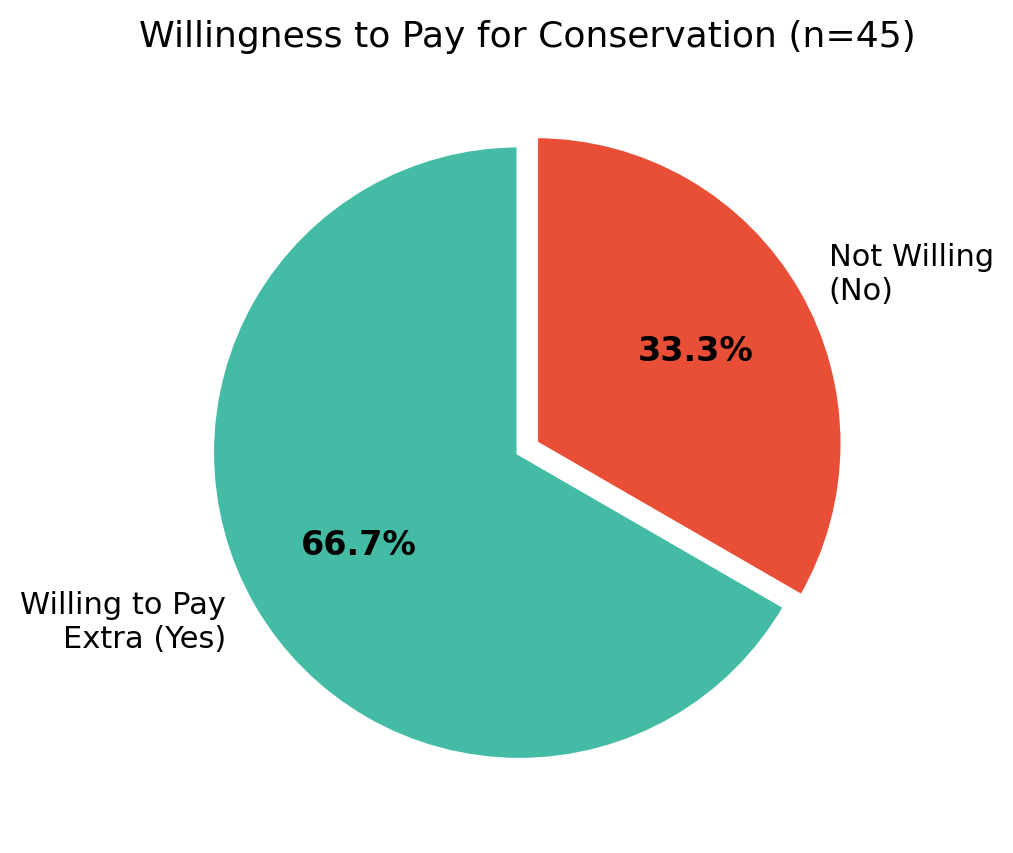
\includegraphics[width=0.85\linewidth]{../report/figures/05_wtp_pie.png}
                \caption{WTP for higher entry fee}
            \end{figure}

            \vspace{-0.3em}
            \begin{center}
                {\large \textbf{66.7\%} said \textcolor{successGreen}{\textbf{Yes}}}\\[4pt]
                {\small 33.3\% said No}
            \end{center}
        \end{column}
        \begin{column}{0.52\textwidth}
            \begin{figure}
                \centering
                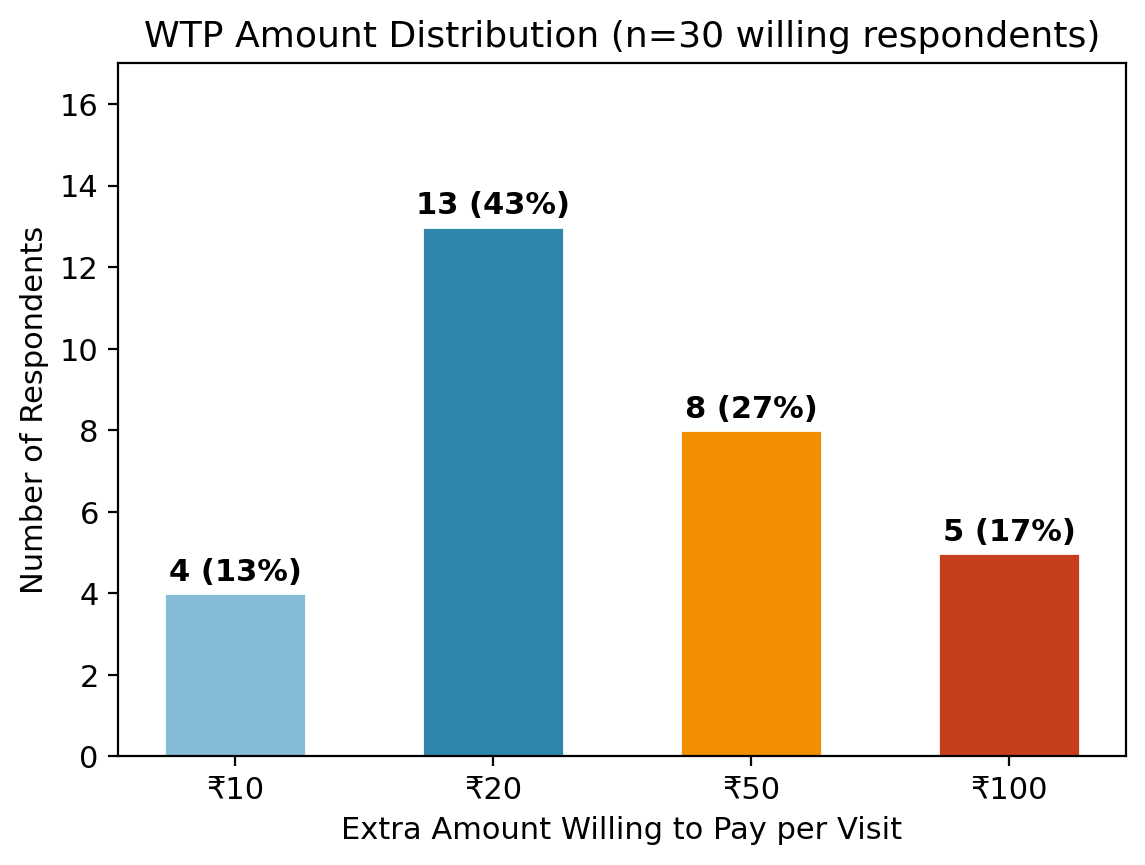
\includegraphics[width=\linewidth]{../report/figures/06_wtp_amount_distribution.png}
                \caption{Max extra amount willing to pay}
            \end{figure}

            \vspace{-0.3em}
            \begin{table}
                \centering
                \scriptsize
                \begin{tabular}{@{}lr@{}}
                    \toprule
                    \textbf{Statistic} & \textbf{Value} \\
                    \midrule
                    Mean WTP (willing) & \rupee 40.0/visit \\
                    Median WTP (willing) & \rupee 20/visit \\
                    Overall Mean WTP & \rupee 26.7/visit \\
                    \textbf{Aggregate annual WTP} & \textbf{\rupee 4.00 crore} \\
                    \bottomrule
                \end{tabular}
            \end{table}
        \end{column}
    \end{columns}
\end{frame}

% ─── SLIDE 10: PROTEST BIDS ──────────────────────────────────────────────
\begin{frame}{Protest Bid Analysis}
    \begin{columns}[T]
        \begin{column}{0.45\textwidth}
            \begin{figure}
                \centering
                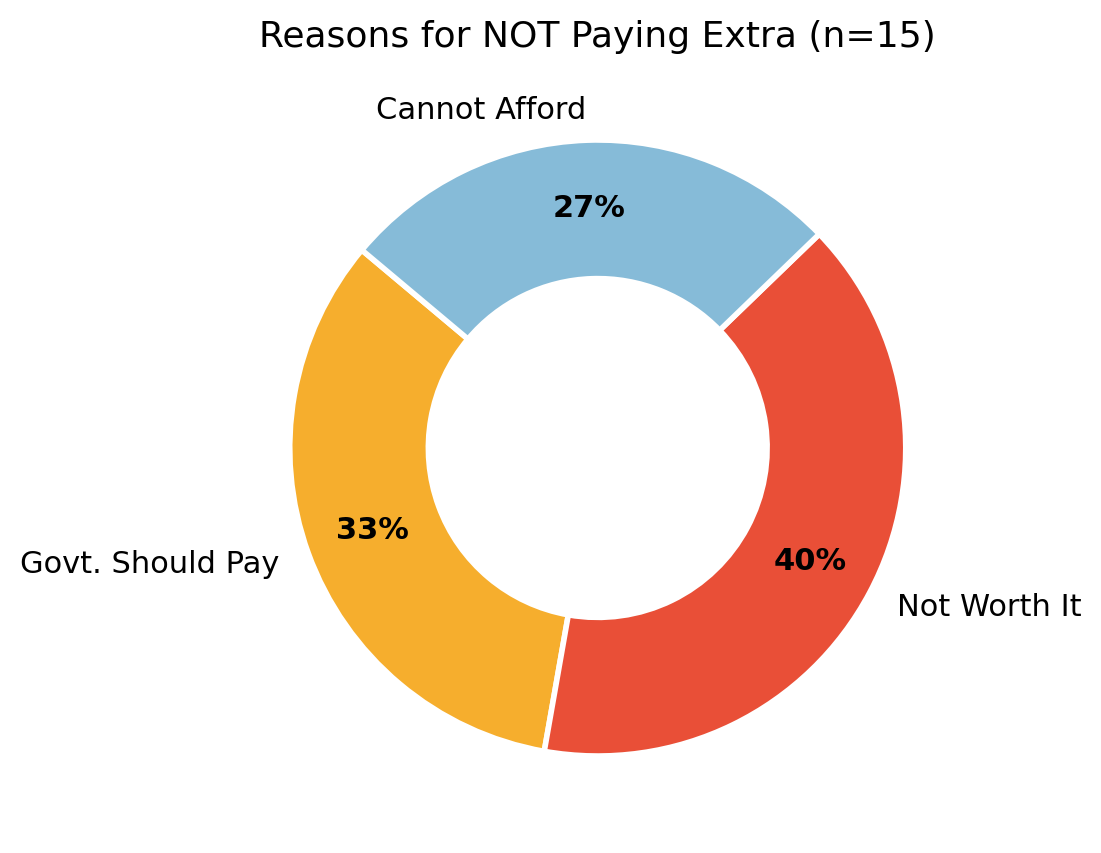
\includegraphics[width=0.9\linewidth]{../report/figures/07_protest_bids.png}
                \caption{Reasons for not paying extra}
            \end{figure}
        \end{column}
        \begin{column}{0.52\textwidth}
            \textbf{Among 15 ``No'' respondents:}
            \begin{itemize}
                \item 40\% - Not worth paying more
                \item 33\% - Govt.\ should bear the cost
                \item 27\% - Cannot afford to pay more
            \end{itemize}

            \vspace{0.6em}
            \begin{alertblock}{Protest Bids}
                \small
                The ``government should pay'' responses (5 respondents) are \textbf{protest bids} - they object to the payment vehicle, not the park's value.\\[6pt]
                Excluding protest bids:\\
                Adjusted WTP rate = $\frac{30}{40}$ = \textbf{75\%}
            \end{alertblock}
        \end{column}
    \end{columns}
\end{frame}

% ─── SLIDE 11: NON-USE VALUES ────────────────────────────────────────────
\begin{frame}{Non-Use Value Analysis}
    \begin{columns}[T]
        \begin{column}{0.48\textwidth}
            \textbf{Bequest Value:}
            \begin{figure}
                \centering
                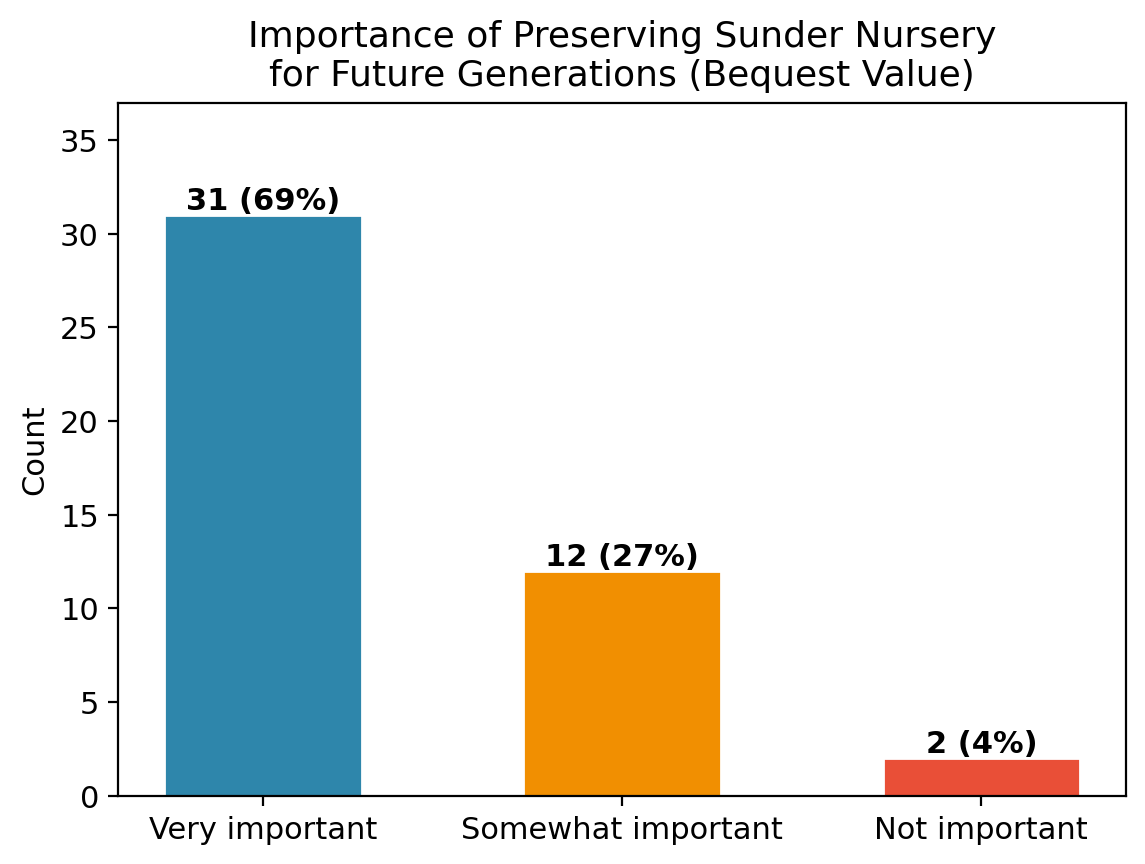
\includegraphics[width=0.85\linewidth]{../report/figures/08_future_importance.png}
                \caption{Importance of preservation for future generations}
            \end{figure}
            \begin{center}
                \small \textbf{68.9\%} said ``Very important''\\
                26.7\% ``Somewhat important''
            \end{center}
        \end{column}
        \begin{column}{0.48\textwidth}
            \textbf{Existence Value:}
            \begin{figure}
                \centering
                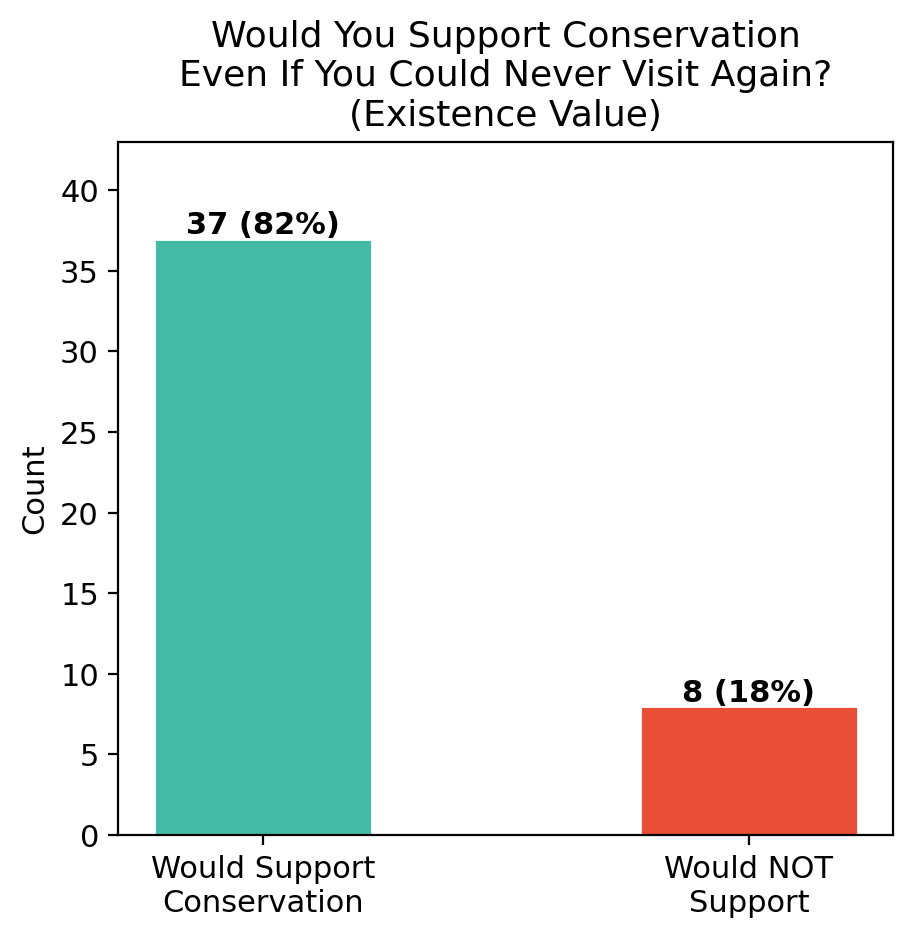
\includegraphics[width=0.85\linewidth]{../report/figures/09_existence_value.png}
                \caption{Support conservation even if never visiting again?}
            \end{figure}
            \begin{center}
                \small \textbf{82.2\%} said Yes
            \end{center}
        \end{column}
    \end{columns}

    \vspace{0.2em}
    \keyinsight{Strong non-use values indicate the park's worth extends far beyond direct recreational use.}
\end{frame}

% ─── SLIDE 12: ECOLOGICAL CONDITION ──────────────────────────────────────
\begin{frame}{Ecological Condition Rating}
    \begin{columns}[T]
        \begin{column}{0.50\textwidth}
            \begin{figure}
                \centering
                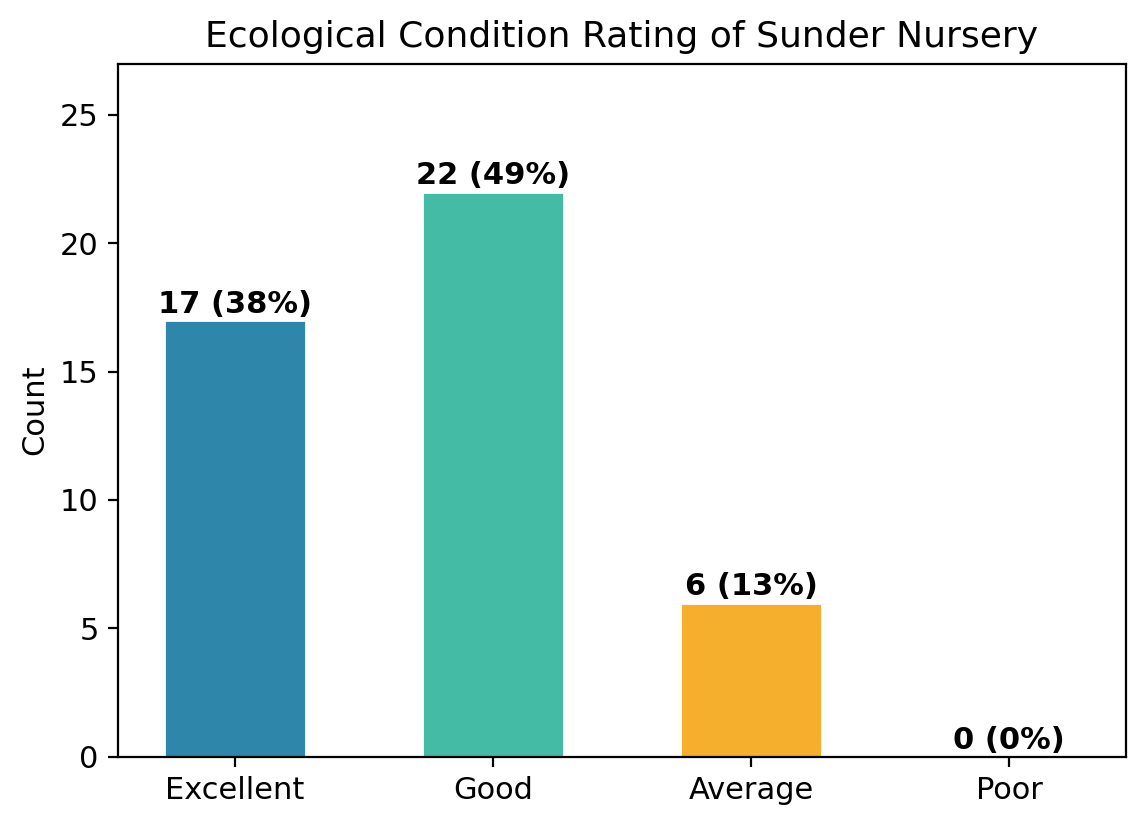
\includegraphics[width=\linewidth]{../report/figures/10_ecological_condition.png}
                \caption{Ecological condition rating by visitors}
            \end{figure}
        \end{column}
        \begin{column}{0.47\textwidth}
            \vspace{1em}
            \textbf{Visitor perception:}
            \begin{itemize}
                \item Excellent: \textbf{37.8\%}
                \item Good: \textbf{48.9\%}
                \item Average: 13.3\%
                \item Poor: 0\%
            \end{itemize}

            \vspace{0.6em}
            \begin{exampleblock}{Validation}
                \small
                \textbf{86.7\%} rate it ``Good'' or ``Excellent'' - validating the Aga Khan Trust restoration program's ecological success.
            \end{exampleblock}
        \end{column}
    \end{columns}
\end{frame}

% ─── SLIDE 13: TCM RESULTS ───────────────────────────────────────────────
\begin{frame}{TCM Results: Travel Cost \& Consumer Surplus}
    \begin{columns}[T]
        \begin{column}{0.48\textwidth}
            \begin{figure}
                \centering
                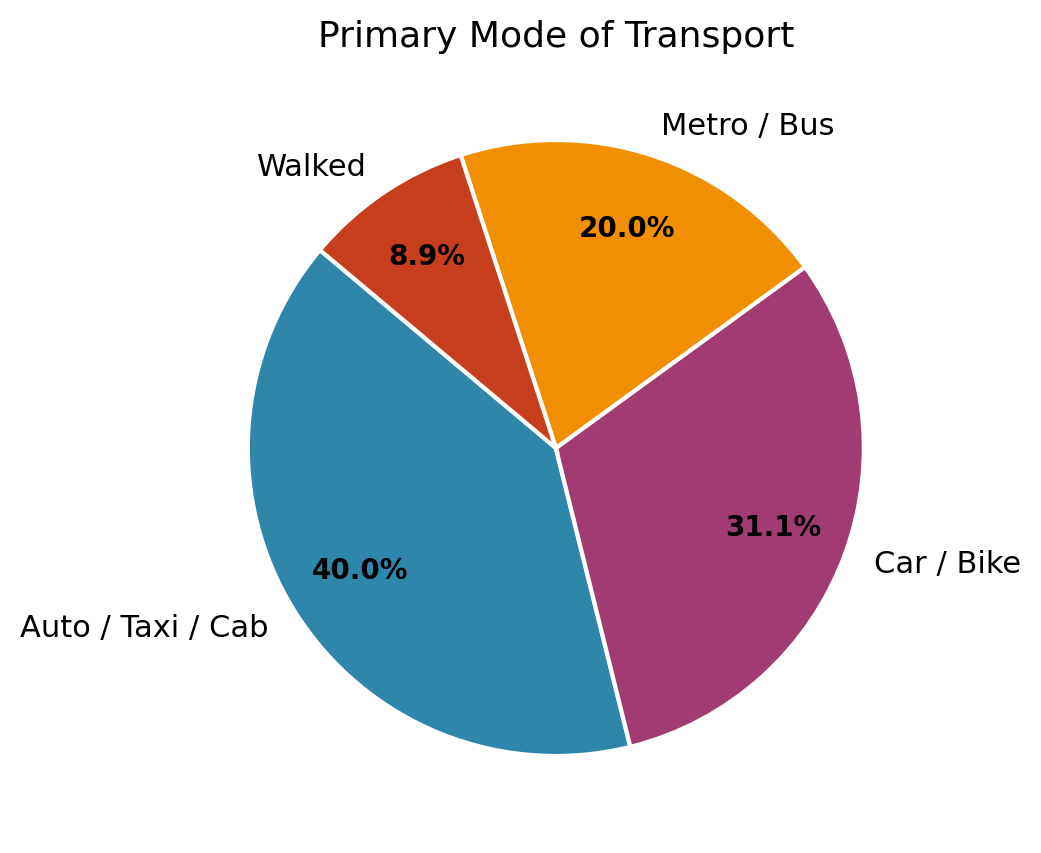
\includegraphics[width=\linewidth]{../report/figures/11_transport_mode.png}
                \caption{Transport mode distribution}
            \end{figure}
            \vspace{-0.5em}
            \begin{figure}
                \centering
                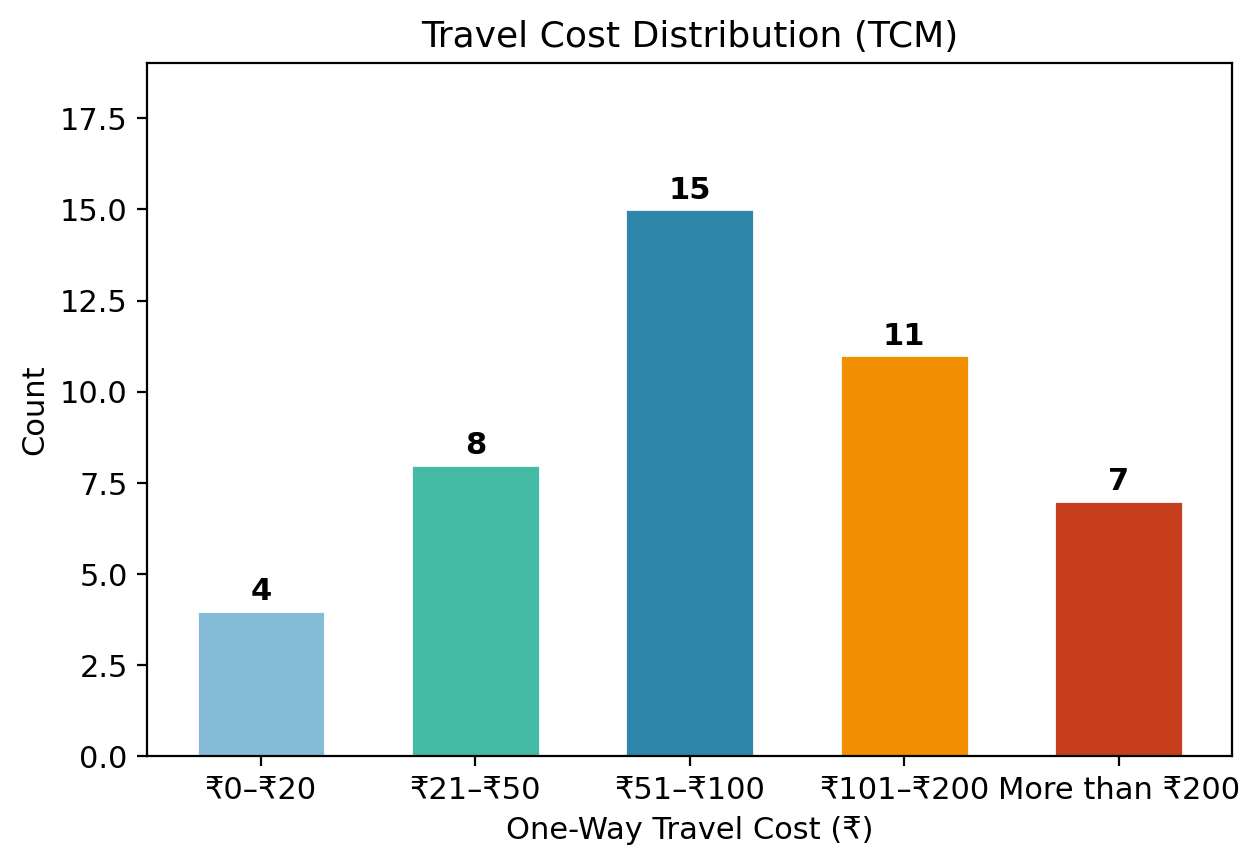
\includegraphics[width=\linewidth]{../report/figures/12_travel_cost.png}
                \caption{One-way travel cost}
            \end{figure}
        \end{column}
        \begin{column}{0.48\textwidth}
            \vspace{0.5em}
            \begin{table}
                \centering
                \small
                \begin{tabular}{@{}lr@{}}
                    \toprule
                    \textbf{Statistic} & \textbf{Value} \\
                    \midrule
                    Mean one-way cost & \rupee 107.7 \\
                    Mean round-trip & \rupee 215.3 \\
                    \textbf{CS per visitor} & \textbf{\rupee 142.3} \\
                    Est.\ annual visitors & $\sim$15 lakh \\
                    \textbf{Annual CS} & \textbf{\rupee 21.35 cr} \\
                    \bottomrule
                \end{tabular}
            \end{table}

            \vspace{0.4em}
            \begin{itemize}
                \small
                \item Auto/taxi most common (40\%)
                \item 53.3\% also visiting nearby sites (Humayun's Tomb)
                \item 51.1\% travel 31-60 min one-way
            \end{itemize}
        \end{column}
    \end{columns}
\end{frame}

% ─── SLIDE 14: DEMAND CURVE ──────────────────────────────────────────────
\begin{frame}{Demand Curve \& Consumer Surplus}
    \begin{columns}[T]
        \begin{column}{0.55\textwidth}
            \begin{figure}
                \centering
                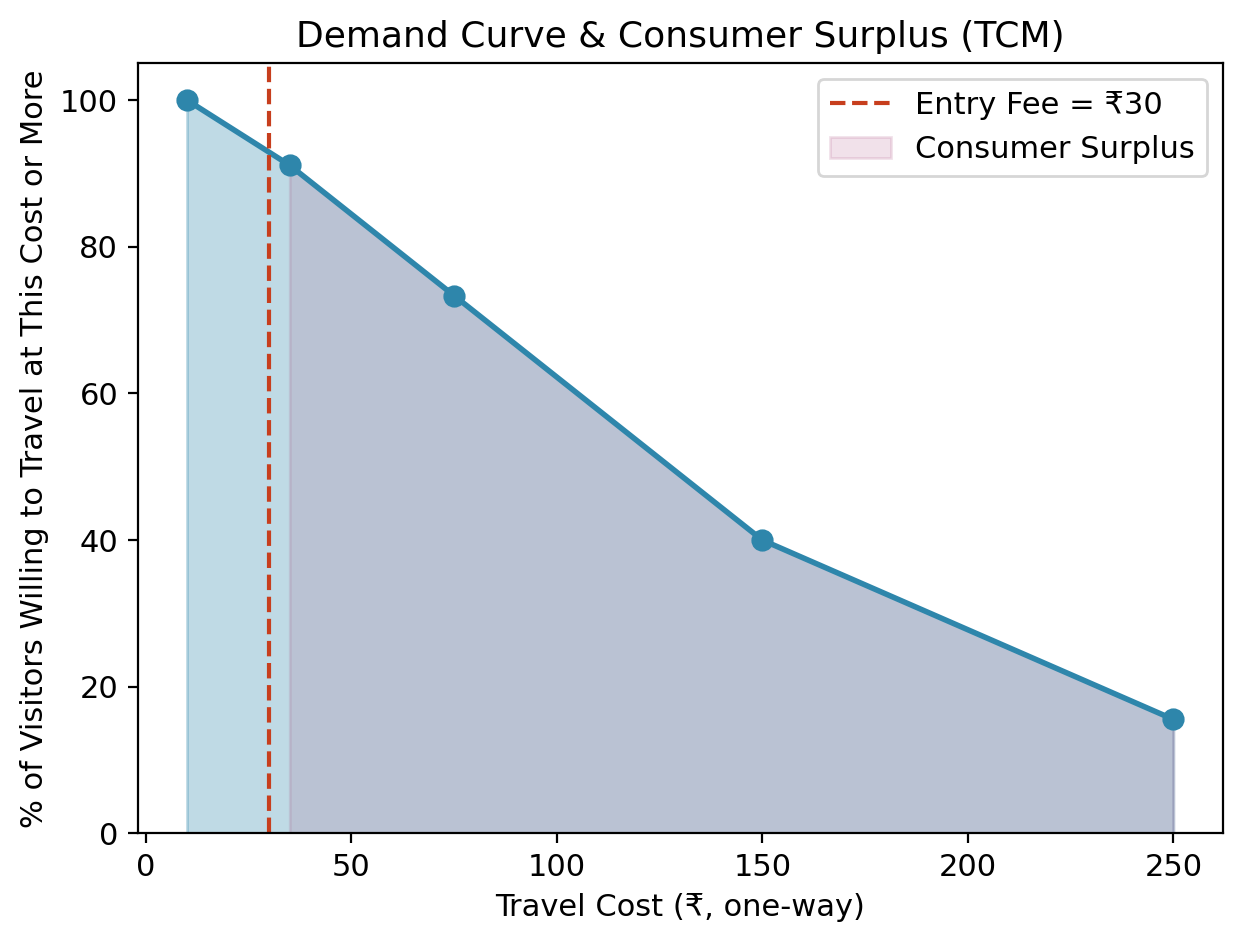
\includegraphics[width=\linewidth]{../report/figures/19_consumer_surplus.png}
                \caption{Demand curve estimated via TCM}
            \end{figure}
        \end{column}
        \begin{column}{0.42\textwidth}
            \vspace{1em}
            \textbf{Interpretation:}
            \begin{itemize}
                \small
                \item Downward-sloping curve confirms theory: higher travel cost $\rightarrow$ fewer visitors
                \item Shaded area = \textbf{consumer surplus} (benefit above actual spend)
                \item Current entry fee (\rupee 20-30) captures only a tiny fraction of the true value
            \end{itemize}

            \vspace{0.5em}
            \keyinsight{Visitors reveal their true valuation through what they spend to get there, not just the entry fee.}
        \end{column}
    \end{columns}
\end{frame}

% ─── SLIDE 15: CROSS-TABULATIONS ─────────────────────────────────────────
\begin{frame}{Cross-Tabulations: Who is Willing to Pay?}
    \begin{columns}[T]
        \begin{column}{0.48\textwidth}
            \begin{figure}
                \centering
                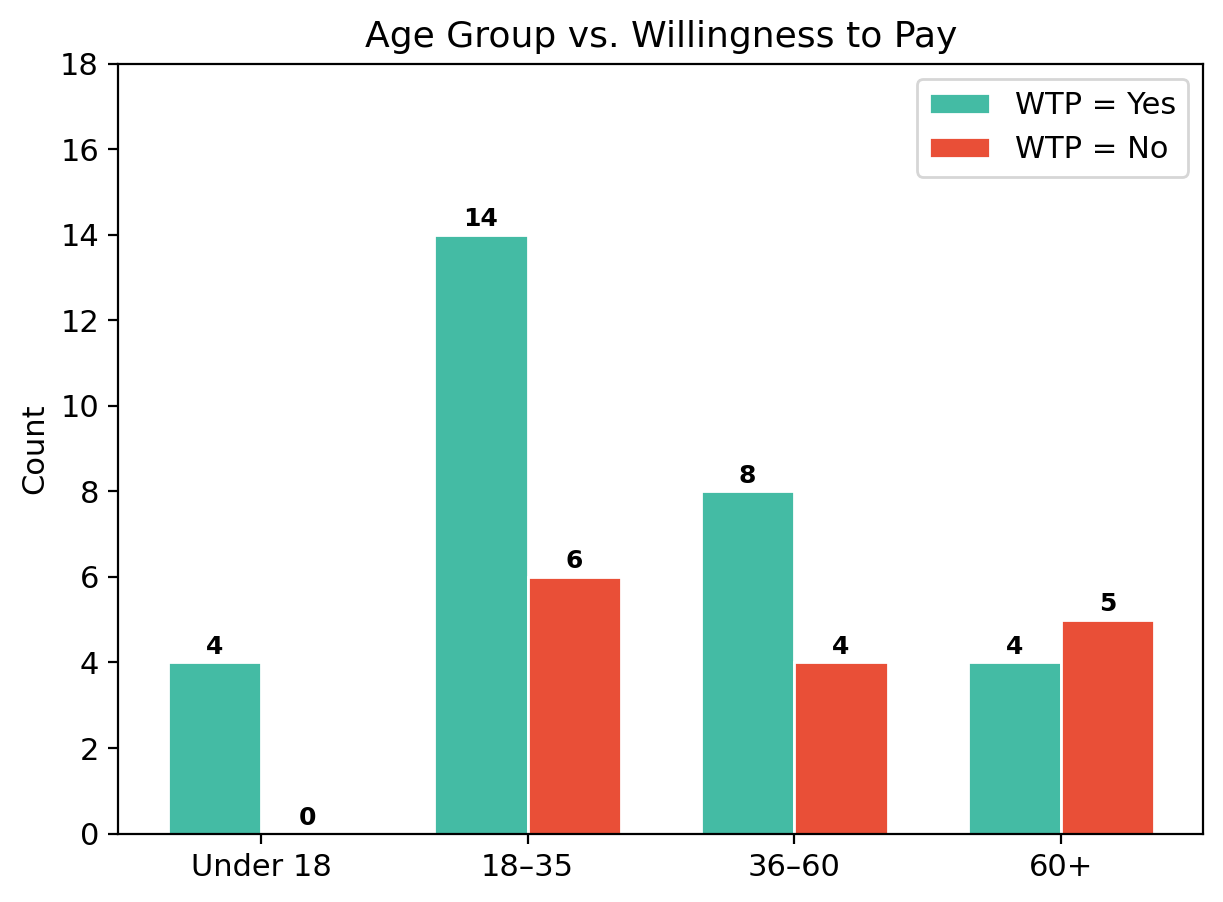
\includegraphics[width=\linewidth]{../report/figures/16_age_vs_wtp.png}
                \caption{Age group vs.\ WTP}
            \end{figure}
            \vspace{-0.3em}
            \small Under 18: 100\% WTP $\rightarrow$ 60+: 44\% WTP
        \end{column}
        \begin{column}{0.48\textwidth}
            \begin{figure}
                \centering
                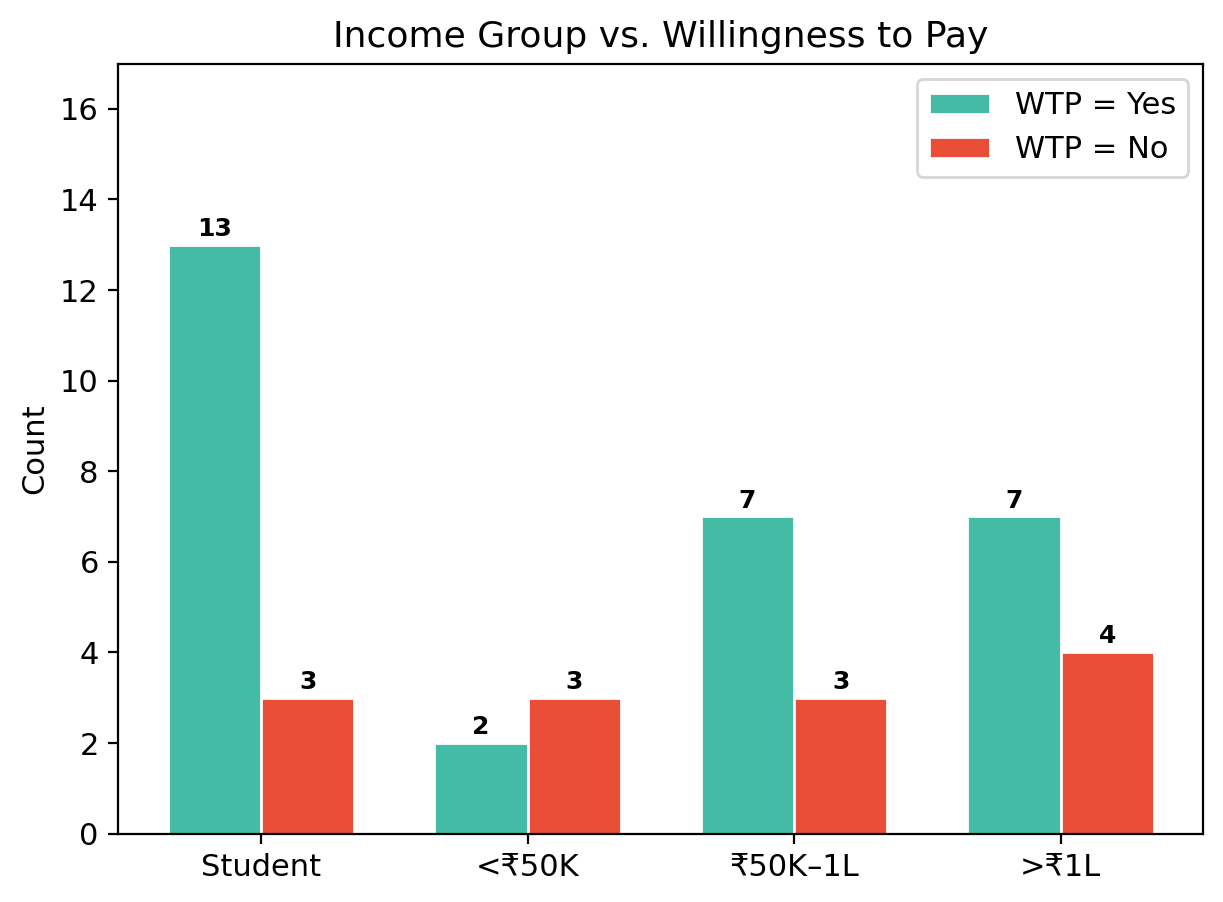
\includegraphics[width=\linewidth]{../report/figures/15_income_vs_wtp.png}
                \caption{Income group vs.\ WTP}
            \end{figure}
            \vspace{-0.3em}
            \small Students: highest WTP (81\%)
        \end{column}
    \end{columns}

    \vspace{0.3em}
    \keyinsight{Environmental concern can outweigh income effects - students show the highest WTP rate despite lower income.}
\end{frame}

% ═══════════════════════════════════════════════════════════════════════════
\section{Total Economic Value}
% ═══════════════════════════════════════════════════════════════════════════

% ─── SLIDE 16: TEV ───────────────────────────────────────────────────────
\begin{frame}{Total Economic Value of Sunder Nursery}
    \begin{columns}[T]
        \begin{column}{0.50\textwidth}
            \begin{table}
                \centering
                \small
                \begin{tabular}{@{}llr@{}}
                    \toprule
                    \textbf{Component} & \textbf{Method} & \textbf{\rupee cr/yr} \\
                    \midrule
                    Use Value (CS) & TCM & 21.35 \\
                    Direct WTP & CVM & 4.00 \\
                    Non-Use Value & CVM $\times$ 0.59 & 2.36 \\
                    \midrule
                    \textbf{Total} & & \textbf{27.71} \\
                    \bottomrule
                \end{tabular}
            \end{table}

            \vspace{0.3em}
            \textbf{Non-use multiplier:}
            \[
                1 + (0.689 \times 0.5) + (0.822 \times 0.3) = 1.59
            \]
            Non-use component: $(1.59 - 1) \times$ \rupee 4.00 = \rupee 2.36 cr
        \end{column}
        \begin{column}{0.47\textwidth}
            \begin{figure}
                \centering
                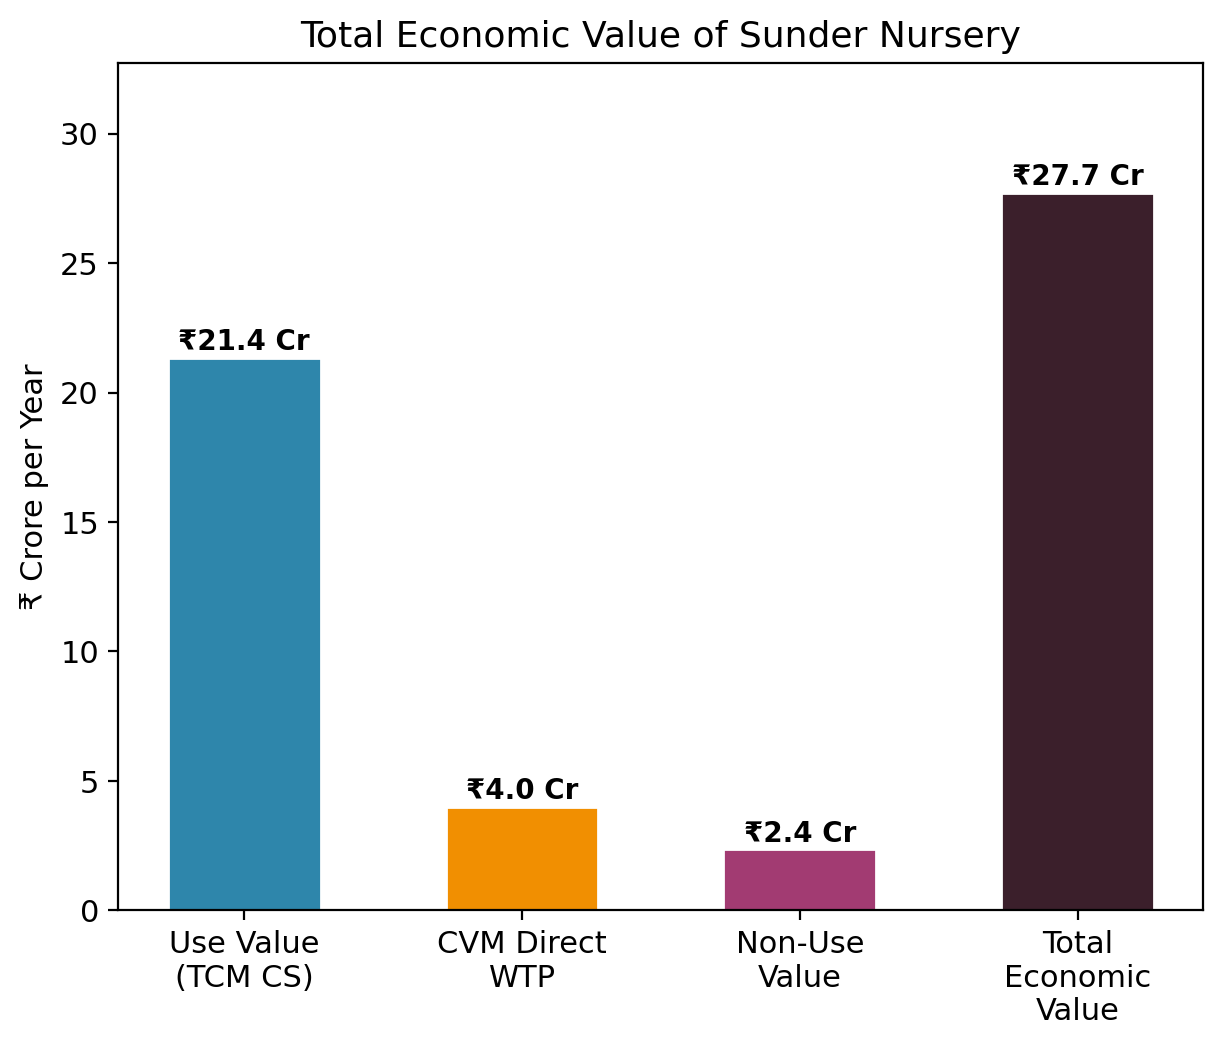
\includegraphics[width=\linewidth]{../report/figures/21_total_economic_value.png}
                \caption{TEV breakdown}
            \end{figure}

            \vspace{-0.2em}
            \begin{alertblock}{}
                \centering
                \small
                \textbf{TEV $\approx$ \rupee 27.71 crore/year}\\[4pt]
                vs.\ entry fee revenue of $\sim$\rupee 3-4.5 crore
            \end{alertblock}
        \end{column}
    \end{columns}
\end{frame}

% ═══════════════════════════════════════════════════════════════════════════
\section{Discussion \& Conclusion}
% ═══════════════════════════════════════════════════════════════════════════

% ─── SLIDE 17: DISCUSSION ────────────────────────────────────────────────
\begin{frame}{Discussion: Comparison \& Policy Implications}
    \begin{columns}[T]
        \begin{column}{0.50\textwidth}
            \textbf{Comparison with Literature:}
            \begin{itemize}
                \small
                \item \textbf{Lumpinee Park, Bangkok} [1]: Non-use values increased capitalized value by $\sim$9$\times$; our multiplier (1.59$\times$) is more conservative
                \item \textbf{Colorado Wilderness} [4]: Non-use = 37\% of total; ours is 8.5\%, reasonable given large TCM use value
                \item Survey design mirrors \textbf{Kalamazoo Nature Center} [7]
            \end{itemize}
        \end{column}
        \begin{column}{0.47\textwidth}
            \textbf{Policy Implications:}
            \begin{enumerate}
                \small
                \item \textbf{Entry fee revision:} A modest \rupee 20-50 increase acceptable to majority; could generate \rupee 3-7.5 cr/yr extra
                \item \textbf{Public investment:} 33\% protest bidders want govt.\ funding - supports continued public investment
                \item \textbf{Youth engagement:} High student WTP suggests outreach programs would strengthen conservation support
            \end{enumerate}
        \end{column}
    \end{columns}
\end{frame}

% ─── SLIDE 18: LIMITATIONS ───────────────────────────────────────────────
\begin{frame}{Limitations}
    \begin{columns}[T]
        \begin{column}{0.48\textwidth}
            \begin{alertblock}{CVM Biases [5]}
                \small
                \begin{enumerate}
                    \item \textbf{Strategic bias:} Free-rider behavior or ``warm glow'' overstating
                    \item \textbf{Hypothetical bias:} No real money changed hands
                    \item \textbf{Information bias:} Limited info in a 2-min survey
                \end{enumerate}
            \end{alertblock}
        \end{column}
        \begin{column}{0.48\textwidth}
            \begin{alertblock}{Sampling Limitations}
                \small
                \begin{enumerate}
                    \setcounter{enumi}{3}
                    \item \textbf{Sample bias:} Single Friday evening; weekday/morning visitors may differ
                    \item \textbf{Small sample:} n = 45; larger surveys (200+) needed for robust policy
                \end{enumerate}
            \end{alertblock}

            \vspace{0.4em}
            \keyinsight{Despite limitations, results are directionally consistent with established literature.}
        \end{column}
    \end{columns}
\end{frame}

% ─── SLIDE 19: CONCLUSION ────────────────────────────────────────────────
\begin{frame}{Conclusion}
    \begin{block}{Key Findings}
        \begin{enumerate}
            \item \textbf{Strong WTP:} 66.7\% willing to pay higher entry fee; mean WTP = \rupee 40/visit
            \item \textbf{Robust non-use values:} 68.9\% bequest (``very important'') + 82.2\% existence value
            \item \textbf{Ecological success:} 86.7\% rate condition as Good/Excellent
            \item \textbf{Significant consumer surplus:} \rupee 142/visitor $\rightarrow$ \rupee 21.35 crore/year
        \end{enumerate}
    \end{block}

    \vspace{0.5em}
    \begin{exampleblock}{}
        \centering
        \large
        \textbf{Total Economic Value $\approx$ \rupee 27.71 crore/year}\\[6pt]
        \small Sunder Nursery's value is largely invisible to the market, but is very much perceived and cherished by those who visit it - and even by those who simply want to know it exists.
    \end{exampleblock}
\end{frame}

% ─── SLIDE 20: REFERENCES ────────────────────────────────────────────────
\begin{frame}{References}
    \small
    \begin{enumerate}
        \item[{[1]}] Dixon, J.A.\ and Hufschmidt, M.M.\ (1986). \textit{Economic Valuation Techniques for the Environment}. Johns Hopkins University Press.
        \item[{[2]}] Krutilla, J.V.\ (1967). Conservation reconsidered. \textit{American Economic Review}, 57(4).
        \item[{[3]}] Johansson, P.O.\ (1990). \textit{The Economic Theory and Measurement of Environmental Benefits}. Cambridge UP.
        \item[{[4]}] Walsh, R.G., Loomis, J.B., and Gillman, R.A.\ (1984). Valuing option, existence, and bequest demands for wilderness. \textit{Land Economics}, 60(1).
        \item[{[5]}] Schulze, W.D., d'Arge, R.C., and Brookshire, D.S.\ (1981). Valuing environmental commodities. \textit{Western J.\ Agric.\ Econ.}, 6(2).
        \item[{[6]}] Aga Khan Trust for Culture (2018). \textit{Sunder Nursery Heritage Park}. New Delhi.
        \item[{[7]}] RDL725 Course Material (Prof.\ Vivek Kumar, IIT Delhi).
    \end{enumerate}
\end{frame}

% ─── SLIDE 21: THANK YOU ─────────────────────────────────────────────────
\begin{frame}[plain]
    
\begin{tikzpicture}[remember picture, overlay]
        \fill[left color=iitdDark, right color=iitdAccent!80!iitdNavy]
            (current page.south west) rectangle (current page.north east);
        \fill[white, opacity=0.06]
            ([xshift=-2cm, yshift=-3cm]current page.north east) circle (7cm);
        \fill[white, opacity=0.04]
            ([xshift=3cm, yshift=2cm]current page.south west) circle (5cm);
    \end{tikzpicture}
    \vfill
    \begin{center}
        {\fontsize{28}{34}\selectfont\bfseries\color{white}Thank You}\\[16pt]
        {\Large\color{white}Open for Questions}\\[20pt]
        {\color{white!70}\rule{5cm}{0.5pt}}\\[20pt]
        {\normalsize\color{white}%
         \textbf{Prem Bhugra}\;\;|\;\;%
         \textbf{Sakhare Yash Balram}\;\;|\;\;%
         \textbf{Ninad Narsing Gawade}\;\;|\;\;%
         \textbf{Nitin Verma}}\\[10pt]
        {\normalsize\color{white!90}%
         Department of Chemical Engineering\\
         Indian Institute of Technology Delhi}
    \end{center}
    \vfill
\end{frame}

\end{document}
